\documentclass[border=2pt]{standalone}
\usepackage{tikz}
\usetikzlibrary{arrows.meta,chains,%
                    decorations.pathreplacing}
\usetikzlibrary{matrix,positioning,arrows.meta,arrows}
\usetikzlibrary{calc}
\usepackage{multirow,array}

\newcommand\hlight[1]{\tikz[overlay, remember picture]\node[rectangle,fill=blue!50,rounded corners,fill opacity = 0.2,draw,thick,text opacity =1] {$#1$};} 

\newcommand\diag[4]{%
%  \multicolumn{1}{p{#2}|}
  \parbox[t]{#2}%
  {\hskip-\tabcolsep
  $\vcenter{\begin{tikzpicture}[baseline=0,anchor=south west,inner sep=#1]
  \path[use as bounding box] (0,0) rectangle (\baselineskip,\baselineskip);
  \node[minimum width={#2+1\tabcolsep},minimum height=\baselineskip+\extrarowheight] (box) {};
%  \draw (box.north west) -- (box.south east);
  \node[anchor=south west] at (box.south) {#3};
  \node[anchor=north east] at (box.east) {#4};
 \end{tikzpicture}}$\hskip-\tabcolsep}}

\tikzset{
mymat/.style={
  matrix of nodes,
  nodes in empty cells,
  text height=2.5ex,
  text depth=0.75ex,
  text width=3.25ex,
  align=center,
  column sep=-\pgflinewidth
  },
cartesian/.style={
  align=center, inner sep=1pt, text centered,
  font=\sffamily, circle, black, draw=black, 
  fill=white, text=black, minimum width=0.5em, minimum height=1em
  }
}
\tikzset{
  rows/.style 2 args={
    sub@rows/.style={row ##1 column #2/.style={nodes={rectangle,draw=black}}},
    sub@rows/.list={#1}
  },
  box/.style 2 args={
    sub@box/.style={rows={#1}{##1}},
    sub@box/.list={#2}
  },
  dsgroup/.style={
    rounded corners=0.5em, 
    fill=blue!50,fill opacity=0.2
  }
}
\begin{document}

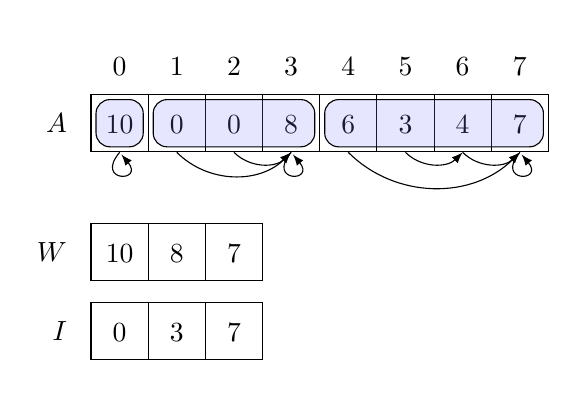
\begin{tikzpicture}[>=latex]
\matrix[mymat,anchor=west,
    box={2}{1, 2, 3, 4, 5, 6, 7, 8}]
at (0,0) 
(mat1)
{ 
   0 & 1 & 2 & 3 & 4 & 5 & 6 & 7\\
  10 & 0 & 0 & 8 & 6 & 3 & 4 & 7\\ };
 
\node[left=5pt of mat1-2-1.west]{$A$};

\matrix[mymat,anchor=west,
    box={1}{1, 2, 3}]
at (0,-2) 
(matw)
{ 
  10 & 8 & 7 \\};

\node[left=5pt of matw-1-1.west]{$W$};

\matrix[mymat,anchor=west,
    box={1}{1, 2, 3}]
at (0,-3)
(mati)
{ 
  0 & 3 & 7  \\};

\node[left=5pt of mati-1-1.west]{$I$};

\draw[dsgroup] 
  ([xshift=2pt, yshift=-2pt]mat1-2-1.north west) rectangle 
  ([xshift=-2pt, yshift=2pt]mat1-2-1.south east) {};

\draw[thin]
  (mat1-2-1.south) edge[in=-50, out=-130, loop] (mat1-2-1.south);

\draw[dsgroup] 
  ([xshift=2pt, yshift=-2pt]mat1-2-2.north west) rectangle 
  ([xshift=-2pt, yshift=2pt]mat1-2-4.south east) {};

\draw[->,thin]
  (mat1-2-2.south) to [bend right=45] (mat1-2-4.south);
\draw[->,thin]
  (mat1-2-3.south) to [bend right=45] (mat1-2-4.south);
\draw[thin]
  (mat1-2-4.south) edge[in=-50, out=-130, loop] (mat1-2-4.south);

\draw[dsgroup] 
  ([xshift=2pt, yshift=-2pt]mat1-2-5.north west) rectangle 
  ([xshift=-2pt, yshift=2pt]mat1-2-8.south east) {};

\draw[->,thin]
  (mat1-2-5.south) to [bend right=45] (mat1-2-8.south);
\draw[->,thin]
  (mat1-2-6.south) to [bend right=45] (mat1-2-7.south);
\draw[->,thin]
  (mat1-2-7.south) to [bend right=45] (mat1-2-8.south);
\draw[thin]
  (mat1-2-8.south) edge[in=-50, out=-130, loop] (mat1-2-8.south);


\end{tikzpicture}

\end{document}